\documentclass[../proyecto.tex]{memoir}

\begin{document}

\chapter{Descripción del contexto}


\section{Representación y actualización del juego de vida de Conway}

%Fijada una configuración inicial $z$, enteremos por ejecución o simulación del juego de vida de Conway de duración $n \in \mathds{N} \cup \{ \infty\}$ al resultado de aplicar $n$ veces la función de transición global del juego de vida de Conway a la configuración inicial y lo notaremos $C_{n}(z)$. Sea $t$ tal que $1 \leq t \leq n$, diremos que es el instante $t$ de la ejecución/simulación/experimento del juego de vida de Conway de duración $t$, el resultado de aplicar $t$ veces la función de transición global a una configuración inicial $z$ y lo notaremos $C^t_n(z)$. Por último, los conjuntos de puntos $C^{t'}_{n'}(z')$, $C^{t}_{n}(z)$ si los conjuntos de células de cada simulación son idénticos. De la misma manera, entederemos por ejecución o simulación del juego de vida de Conway $\alpha$-asíncrono de duración $n$ al resultado de aplicar $n$ veces la función de transición global a la configuración inicial $z$ y lo notaremos $C_{n}(z)(\alpha)$ donde $\alpha$ es un número real en el intervalo $(0,1)$.

Como se comentaba en la introducción, plantearse la simulación del juego de vida implica afrontar el problema de representar una malla infinita de dos dimensiones en la memoria finita de los ordenadores. Mientras que la cantidad de memoria y velocidad de acceso de la misma ha mejorado significativamente con el paso del tiempo, perseguimos una representación que cumpla las siguientes dos características:

\begin{itemize}
\item Una simulación de una configuración inicial del juego de vida tiene que finalizar en un tiempo razonable, pues la clave de los métodos Monte Carlo son la repetición de las mismas y como se comenta posteriormente en \ref{carlino}, al aumentar el número de simulaciones disminuye la varianza, permitiendo mayor precisión.

\item El comportamiento de las configuraciones iniciales es difícil de predecir, por lo que aquellas que crezcan sin límite podrían agotar los recursos de memoria disponibles haciendo que la ejecución sea inválida. En particular, una situación con alto consumo de memoria dificulta la ejecución de múltiples simulaciones independientes en paralelo.
\end{itemize}

Este último punto es, en nuestra opinión, el más restrictivo. Un planteamiento inicial nos podría sugerir que limitar el tamaño de la malla dos dimensional, sin embargo se perdería información en aquellas configuraciones iniciales que excedieran el tamaño fijado de la malla. Para reducir el impacto de la finitud de la malla se ha estudiado la identificación de los bordes opuestos simulando un espacio \textit{infinito} que imita la superficie de un toro, obteniendo resultados favorables \cite{finitudMalla, finitudMalla2}. Pero no es necesario lidiar con los errores derivados de este planteamiento. Una implementación en nuestra opinión más \textit{literal} de la descripción formal del juego de vida, nos permite romper con el paradigma de la limitación de la malla. En lugar de almacenar en memoria la malla completa independientemente de su utilización, se almacenan las células dadas por coordenadas sobre la malla rectangular identificada con el plano cartesiano \cite{boardless}. 

Si suponemos que la malla dos dimensional con los bordes opuestos identificados es cuadrada con lado de tamaño $m$, la complejidad en espacio viene dada por $O(m^2)$ independientemente a la configuración inicial escogida. Por otro lado si suponemos una malla dos dimensional infinita, una configuración inicial con $c$ células y $c(t)$ el número de células en el instante $t$, la complejidad en espacio para cada instante $t$ es $O(c(t))$ y la complejidad en espacio de $C_n^t$ es $O(\max_{0\leq t\leq n}\{c(t)\})$. Así al optar por la implementación de la malla infinita haremos un uso más eficiente de la memoria disponible. Con dicha implementación el vecindario de una célula se calcula sumando a sus coordenadas $(x,y)$ a cada uno de los puntos de este conjunto $\{(-1, 1),\ (0, 1),\ (1, 1),\ (-1, 0),\ (1, 0),\ (-1,-1),\ (0,-1),\ (1,-1)\}$:

\begin{align*}
\begin{array}{lcr}
(x,\ y)+(-1,\ 1) & (x,\ y)+(0,\ 1) & (x,\ y)+(1,\ 1)\\
(x,\ y)+(-1,\ 0) & (x,\ y) & (x,\ y)+(1,\ 0)\\
(x,\ y)+(-1,-1) & (x,\ y)+(0,-1) & (x,\ y)+(1,-1)\\
\end{array} 
\end{align*}

Una vez calculado el vecindario de una célula, las células vivas en el vecindario se calculan como la intersección del vecindario con el conjunto de células vivas. Esta operación es de tiempo constante si se almacenan tanto las células vivas como el vecindario en estructuras de datos de tiempo de búsqueda constante, esto son, tablas hash. Tras el conteo de células vivas en el vecindario de una célula dada, es suficiente con aplicar la tabla de transición de estados \ref{tab:estados} para determinar el siguiente estado de la célula.

\begin{table}[]
\centering
\begin{tabular}{|l|c|c|c|c|c|c|c|c|c|}
\hline
Estado actual           & \multicolumn{9}{c|}{Siguiente estado}  \\ \hline
\multirow{2}{*}{}       & \multicolumn{9}{c|}{Número de vecinos} \\ \cline{2-10} 
                        & 0   & 1  & 2  & 3  & 4 & 5 & 6 & 7 & 8 \\ \hline
\multicolumn{1}{|c|}{0} & 0   & 0  & 0  & 1  & 0 & 0 & 0 & 0 & 0 \\ \hline
\multicolumn{1}{|c|}{1} & 0   & 0  & 1  & 1  & 0 & 0 & 0 & 0 & 0 \\ \hline
\end{tabular}
\caption{Tabla de transición de estados del juego de vida de Conway}
\label{tab:estados}
\end{table}

\section{Representación y actualización del juego de vida de Conway $\alpha$-asíncrono}

Los comentarios realizados en la sección anterior son aplicables al juego de vida de Conway \textit{síncrono}, sin embargo para el juego $\alpha$-asíncrono hay que introducir una pequeña variación en el mecanismo de actualización que vamos a exponer en esta sección. Notar que la descripción de la representación interna de la malla comentada anteriormente se reutiliza en el juego $\alpha$-asíncrono, es decir, la perturbación introducida en la actualización no afecta a la malla rectangular.

En un juego de vida $\alpha$-asíncrono cada célula tiene probabilidad $\alpha$ de ser actualizada y probabilidad $1-\alpha$ de mantener su estado actual, esto es, tiene probabilidad $\alpha$ de que se le aplique la tabla de transición de estados \ref{tab:estados}. A cada célula se le dota la capacidad de generar números pseudo-aleatorios de una distribución uniforme estándar. De esta manera cuando se va a consultar la tabla de transición de estados genera un número aleatorio, si éste es superior a $\alpha$ entonces consulta la tabla y en caso contrario no lo hace, manteniendo su estado actual.

\section{Configuraciones iniciales del juego de vida de Conway} \label{zoo}

Dado que las configuraciones iniciales son muy diversas, han existido algunos esfuerzos por realizar una taxonomía de patrones pero no existe un consenso global y como consecuencia aceptamos la existencia de principalmente tres categorías. En este trabajo trataremos de caracterizar el comportamiento de configuraciones iniciales del juego de vida de Conway bajo la hipótesis de actualización $\alpha$-asíncrona. Nuestras elecciones de patrones está inicialmente motivada por la simplicidad de los mismos, que nos permite visualizar el impacto de la $\alpha$-asincronismo en la actualización. %y a continuación verificar si esta caracterización es extensible a todas las configuraciones iniciales de la misma categoría. 

\subsection{Vidas inmóviles}
Probablemente las vidas inmóviles sean las configuraciones con el comportamiento más simple y fácil de observar. Esta sección está extraída de las siguientes fuentes: \cite{stillLifeProblem},\cite{stillLifeTheory} y \cite{LikeWikiStill}.

%\begin{defi}
%Una vida inmóvil es una configuración inicial que permanece en cada iteración, esto es, fijado $n\in\mathds{N}$, se verifica que $z = C^n_0(z) = C^n_t(z)$ para todo $t \leq n$.
%\end{defi}

\begin{defi}
Una vida inmóvil es una configuración inicial que permanece inmutada en cada iteración.
\end{defi}

Distinguimos tres tipos de vidas inmóviles:

\begin{defi}
Una vida inmóvil estricta es aquella vida inmóvil tal que al eliminar una de sus células vivas deja de ser una vida inmóvil.
\end{defi}

A continuación mostramos ejemplos de estos tipos de vidas inmóviles en la \autoref{fig:congIniciales}. La \autoref{fig:2-1} es una vida inmóvil estricta pues todos los elementos dependen entre sí los unos de los otros, la \autoref{fig:2-2} nuevo es también una vida inmóvil estricta a pesar de que contenga a otra vida inmóvil estricta y la \autoref{fig:2-3} es también una vida inmóvil estricta pues el patrón de la mitad horizontal derecha conserva su estabilidad gracias a su homólogo reflejado de la mitad horizontal izquierda y al alterar el estado de cualquier célula viva se pierde la estabilidad.

\begin{figure}[H]
	\centering
	\begin{subfigure}[b]{0.3\linewidth} 
        \centering
        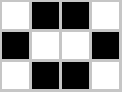
\includegraphics[height=.45\linewidth]{./images/beehive.png}
        \caption{}
        \label{fig:2-1}
    \end{subfigure}
    \quad
	\begin{subfigure}[b]{0.3\linewidth} 
        \centering
        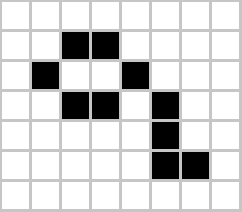
\includegraphics[height=.5\linewidth]{./images/beehive_with_tail.png}
        \caption{}
        \label{fig:2-2}
    \end{subfigure}
	\\    
    \begin{subfigure}[b]{0.3\linewidth} 
        \centering
        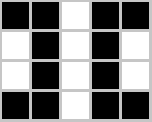
\includegraphics[height=0.5\linewidth]{./images/table_on_table.png}
        \caption{}
        \label{fig:2-3}
    \end{subfigure}
	\caption{Ejemplos de vidas inmóviles estrictas del juego de vida de Conway.}
	\label{fig:congIniciales}
\end{figure} 

\begin{defi}
Una vida pseudo inmóvil es una vida inmóvil que puede ser particionada en vidas inmóviles independientes, es decir, la estabilidad de una de ellas no depende de la presencia de las otras. Además debe de existir al menos una célula muerta por superpoblación (más de tres vecinos vivos) que al particionar en vidas inmóviles independientes la célula continúe muerta por soledad (menos de tres vecinos vivos).
\end{defi}

Las vidas inmóviles que particionan a una vida pseudo inmóvil pueden ser a su vez vidas pseudo inmóviles \autoref{fig:bisnake} o vidas inmóviles estrictas \autoref{fig:biblock}. Notar que una vida inmóvil puede estar formada por varias vidas inmóviles y aún así ser una vida estrictamente inmóvil (y no pseudo inmóvil) en caso de que dependan entre sí para mantener su estabilidad como en la \autoref{fig:2-3}.

\begin{figure}[H]
	\centering
	\begin{subfigure}[b]{0.3\linewidth} 
        \centering
        
\includegraphics[height=.35\linewidth]{./images/biblock.png}
        \caption{}
        \label{fig:biblock}
    \end{subfigure}
    \quad
	\begin{subfigure}[b]{0.3\linewidth} 
        \centering
        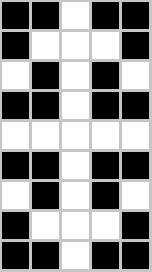
\includegraphics[height=\linewidth]{./images/bisnake.png}
        \caption{}
        \label{fig:bisnake}
    \end{subfigure}
	\caption{Ejemplos de vidas pseudo inmóviles del juego de vida de Conway.}
	\label{fig:congIniciales2}
\end{figure} 

\begin{defi}
Una vida quasi inmóvil es una vida inmóvil que puede ser particionada en vidas inmóviles independientes, es decir, la estabilidad de una de ellas no depende de la presencia de las otras. Además existen células que tanto en la configuración inicial como en las vidas inmóviles independientes se mantengan muertas por soledad (menos de tres vecinos vivos). 
\end{defi}

Notar que la \autoref{fig:biblock} no es una vida quasi inmóvil y sin embargo \autoref{fig:bimoved} sí. Este tipo de vida inmóvil está habitualmente formada por dos vidas inmóviles que comparten una diagonal.

\begin{figure}[H]
	\centering
	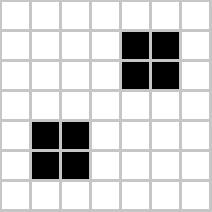
\includegraphics[height=.2\linewidth]{./images/bimoved.png}
	\caption{Configuración inicial que en el centro tiene una célula que se mantiene muerta por soledad tanto en las vidas inmóviles independientes como en el total.}
	\label{fig:bimoved}
\end{figure} 

Por último, cabría preguntarse el problema de dado un número finito de células, ¿cuántas vidas inmóviles existen? Dicho problema ha sido resuelto para vidas inmóviles estrictas y pseudo inmóviles de hasta 32 células, como se puede consultar en \cite{countStillLifes} y en \cite{countPseudoStillLifes}.

\subsection{Osciladores}

%\begin{defi}
%Un oscilador es una configuración inicial $z$ finita y no vacía que se repite tras la aplicación de $k$ veces de la función de transición global, esto es, fijado $n\in\mathds{N}$, se verifica que existe $k>1, \in\mathds{N}$ tal que $C^n_t(z) = C^n_{t+k}(z)$ para todo $t \leq n-k$ y diremos que $k$ es el periodo del oscilador.
%\end{defi}

\begin{defi}
Un oscilador es una configuración inicial que tras un número fijo de iteraciones se repite en la misma posición, al número de iteraciones se le conoce por periodo del oscilador.
\end{defi}

Notar que las vidas inmóviles pueden ser interpretadas como osciladores de periodo una iteración.

En la \autoref{fig:congIniciales3} mostramos dos configuraciones iniciales de periodo dos, a lo largo de tres iteraciones. Por un lado la \autoref{fig:blinker1}, \autoref{fig:blinker2} y \autoref{fig:blinker3} son tres iteraciones de la configuración inicial nombrada \textit{blinker} y por otro la \autoref{fig:toad1}, \autoref{fig:toad2} y \autoref{fig:toad3} son tres iteraciones de la configuración inicial \textit{toad}.

\begin{figure}[H]
	\centering
	\begin{subfigure}[b]{0.3\linewidth} 
        \centering
        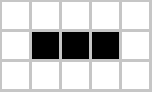
\includegraphics[height=.35\linewidth]{./images/blinker1.png}
        \caption{}
        \label{fig:blinker1}
    \end{subfigure}
    \ 
	\begin{subfigure}[b]{0.3\linewidth} 
        \centering
        
\includegraphics[height=.45\linewidth]{./images/blinker2.png}
        \caption{}
        \label{fig:blinker2}
    \end{subfigure}
    \ 	
    \begin{subfigure}[b]{0.3\linewidth} 
        \centering
        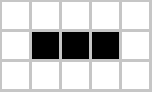
\includegraphics[height=.35\linewidth]{./images/blinker3.png}
        \caption{}
        \label{fig:blinker3}
    \end{subfigure}
    \\
	\begin{subfigure}[b]{0.3\linewidth} 
        \centering
        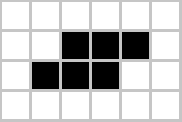
\includegraphics[height=0.35\linewidth]{./images/toad1.png}
        \caption{}
        \label{fig:toad1}
    \end{subfigure}
	\begin{subfigure}[b]{0.3\linewidth} 
        \centering
        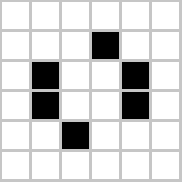
\includegraphics[height=0.45\linewidth]{./images/toad2.png}
        \caption{}
        \label{fig:toad2}
    \end{subfigure}
	\begin{subfigure}[b]{0.3\linewidth} 
        \centering
        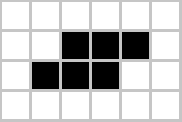
\includegraphics[height=0.35\linewidth]{./images/toad3.png}
        \caption{}
        \label{fig:toad3}
    \end{subfigure}
	\caption{Ejemplos de osciladores de periodo dos del juego de vida de Conway.}
	\label{fig:congIniciales3}
\end{figure} 

\subsection{Naves espaciales}

%\begin{defi}
%Una  nave espacial es una configuración inicial $z$ finita y no vacía que se repite tras la aplicación de $k$ veces de la función de transición global pero en una posición distinta, esto es, fijado $n\in\mathds{N}$, se verifica que existen $k\in\mathds{N}$ y una traslación distinta de la identidad, $\phi:\mathds{Z}^2\to\mathds{Z}^2$, tal que $C^n_t(z) = \phi(C^n_{t+k}(z))$ para todo $t \leq n-k$ y diremos que $k$ es el periodo de la nave espacial.
%\end{defi}

\begin{defi}
Una  nave espacial es una configuración inicial es una configuración inicial que tras un número fijo de iteraciones se repite pero en una posición desplazada.
\end{defi}

Dado que este tipo de configuraciones iniciales se desplaza sobre la malla rectangular es interesante medir la velocidad con la que lo hacen. Si una configuración inicial se desplaza $(x, y)$ unidades cada periodo de longitud $n$, la velocidad de desplazamiento de la nave espacial es: $$
 v = \frac{\max\{|x|,|y|\}c}{k}
 $$  y su pendiente es $x/y$, donde $c$ es la velocidad máxima teórica, un desplazamiento por iteración. Curiosamente se ha demostrado que para cada pendiente existe una nave espacial con dicha pendiente \cite{pendienteNaves}.

En la \autoref{fig:congIniciales4} encontramos dos naves espaciales que se desplazan en distintas direcciones. La \autoref{fig:glider} es la nave espacial más pequeña conocida de velocidad $c/4$ y su desplazamiento es diagonal y la \autoref{fig:lightweightspaceship} es la más pequeña conocida de velocidad $c/2$ y su desplazamiento es horizontal.

\begin{figure}[H]
	\centering
	\begin{subfigure}[b]{0.3\linewidth} 
        \centering
        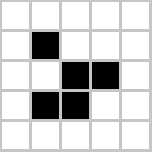
\includegraphics[height=.35\linewidth]{./images/glider.png}
        \caption{}
        \label{fig:glider}
    \end{subfigure}
    \quad
	\begin{subfigure}[b]{0.3\linewidth} 
        \centering
        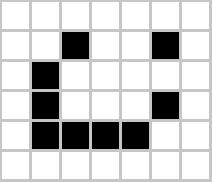
\includegraphics[height=0.45\linewidth]{./images/lightweightspaceship.png}
        \caption{}
        \label{fig:lightweightspaceship}
    \end{subfigure}
	\caption{Ejemplos de vidas pseudo inmóviles del juego de vida de Conway.}
	\label{fig:congIniciales4}
\end{figure} 

\subsection{Selección de configuraciones iniciales}

Los primeros censos de configuraciones iniciales fueron \textit{The Online Life-Life CA Soup Search} y \textit{Achim Flammenkamp's census}, en los que se contabilizaron 174.631.866.050 y 50.158.095.316 configuraciones del juego de vida, respectivamente. El primero de ellos consistió en la evolución de 6.412.048.029 configuraciones iniciales aleatorias que cubren un cuadrado de lado 20 con densidad inicial de 0.5 sobre una malla rectangular infinita \cite{sopa1}. El segundo exploró la evolución de 1.829.196 configuraciones iniciales aleatorias sobre una malla cuadrada de lado 2048 con los bordes opuestos identificados y con una densidad inicial de 0.375 \cite{sopa2}. De ambos censos se puede extraer la conclusión de que las configuraciones que aparecen más a menudo son las vidas inmóviles, seguidas por los osciladores y por último las naves espaciales.

Para nuestro trabajo tomaremos de referencia el censo más actual \textit{Catalogue} que recoge las ejecuciones de 19.640.649.096.999 configuraciones iniciales aleatorias cuadradas de lado 16 del juego de vida de Conway. Se han obtenido un total de 429.049.899.985.558 patrones de los cuales se encontraron 161.861 tipos diferentes \cite{sopa3}. En la tabla \autoref{tab:sopa1naves} se muestran las primeras 5 naves espaciales más frecuentes, las cuales escogeremos para realizar nuestro experimento. Destacar que todas son de periodo 4 y que no tomaremos más dado que el número de ocurrencias disminuye drásticamente de la cuarta a la quitan posición. En la \autoref{fig:congIniciales5} podemos observar la forma de estas configuraciones iniciales. Como representantes de la categoría de osciladores estudiaremos los dos osciladores más frecuente de periodo 2, 3 y 4.

\begin{table}[]
\centering
\begin{tabular}{|l|l|l|l|}
\hline
Ranking & Nombre                          & Periodo & Ocurrencias    \\ \hline
1       & \textit{Glider}                 & 4       & 37.699.263.597.381 \\ \hline
2       & \textit{Lightweight spaceship}  & 4       & 55.075.316.989     \\ \hline
3       & \textit{Middleweight spaceship} & 4       & 14.511.262.233      \\ \hline
4       & \textit{Heavyweight spaceship}  & 4       & 2.521.819.486      \\ \hline
5       & \textit{MWSS on MWSS}  & 4       & 7.077      \\ \hline
\end{tabular}
\caption{Naves espaciales más frecuentes}
\label{tab:sopa1naves}
\end{table}

\begin{figure}[H]
	\centering
	\begin{subfigure}[b]{0.3\linewidth} 
        \centering
        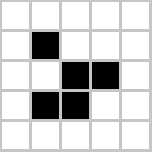
\includegraphics[height=.45\linewidth]{./images/glider.png}
        \caption{\textit{Glider}}
        \label{fig:glider}
    \end{subfigure}
    \ 
	\begin{subfigure}[b]{0.3\linewidth} 
        \centering
        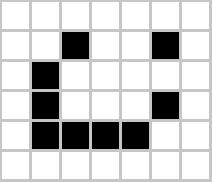
\includegraphics[height=0.45\linewidth]{./images/lightweightspaceship.png}
        \caption{\textit{Lightweight spaceship}}
        \label{fig:lightweightspaceship}
    \end{subfigure}
    \
	\begin{subfigure}[b]{0.3\linewidth} 
        \centering
        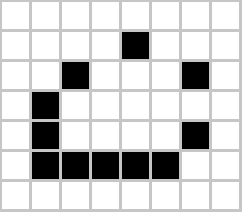
\includegraphics[height=0.45\linewidth]{./images/middleweightspaceship.png}
        \caption{\textit{Middleweight spaceship}}
        \label{fig:middleweightspaceship}
    \end{subfigure}
    \\
	\begin{subfigure}[b]{0.3\linewidth} 
        \centering
        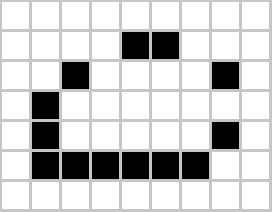
\includegraphics[height=0.45\linewidth]{./images/heavyweightspaceship.png}
        \caption{\textit{Heavyweight spaceship}}
        \label{fig:heavyweightspaceship}
    \end{subfigure}
    \
	\begin{subfigure}[b]{0.3\linewidth} 
        \centering
        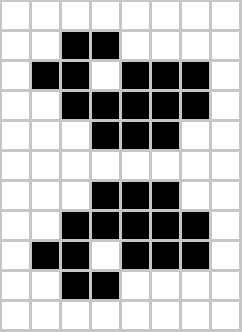
\includegraphics[height=0.65\linewidth]{./images/MWSS_on_MWSS.png}
        \caption{\textit{MWSS on MWSS}}
        \label{fig:mwss2}
    \end{subfigure}
	\caption{Top 5 naves espaciales más frecuentes en el censo {Catalogue}.}
	\label{fig:congIniciales5}
\end{figure} 


% aquí hay que exponer que se descartan las vidas inmóviles porque no se ven afectadas por la perturbación de la actualización

\section{Características medidas sobre las simulaciones}

Dado el carácter aleatorio del juego de vida $\alpha$-asíncrono emplearemos los fundamentos de Monte Carlo expuestos en la sección \ref{MonteCarlo} para medir los parámetros de interés que a continuación exponemos. Nuestras variables de interés son:

\begin{itemize}
\item Crecimiento de la población de células de la configuración inicial: dispondremos de dos herramientas para medir el número de células. Estudiaremos la evolución del número de células en cada etapa, la evolución del área del rectángulo de menor tamaño que contenga a todas las células de cada etapa y su densidad, esto es, el cociente del número de células entre el área anterior.
\item Tasa de cambio de la configuración inicial: emplearemos el concepto de calor, el número de células que nacen o mueren por generación.
\item Distribución de las células en cúmulos: contabilizaremos el número de cúmulos por cada generación, entendiendo por cúmulo al mayor conjunto de células cuyo vecindario no es disjunto, es decir, en un cúmulo cada célula está contenida en el vecindario de otra célula del cúmulo.
\end{itemize}

Estas variables serán medidas para distintos valores de $\alpha$ con el fin de estudiar el efecto de la aleatoriedad en las configuraciones iniciales. Notar que el número de simulaciones realizadas para cada patrón será variable puesto que algunos patrones son de mayor tamaño y en consecuencia tienen simulaciones más lentas.

% Características a medir si sobra tiempo: simulaciones utilizando cadenas de markov y métodos de monte carlo



\end{document}